\section{Quick\_\-String\_\-Hash  Class Reference}
\label{classQuick__String__Hash}\index{Quick_String_Hash@{Quick\_\-String\_\-Hash}}
{\tt \#include $<$dil2al.hh$>$}

Inheritance diagram for Quick\_\-String\_\-Hash::\begin{figure}[H]
\begin{center}
\leavevmode
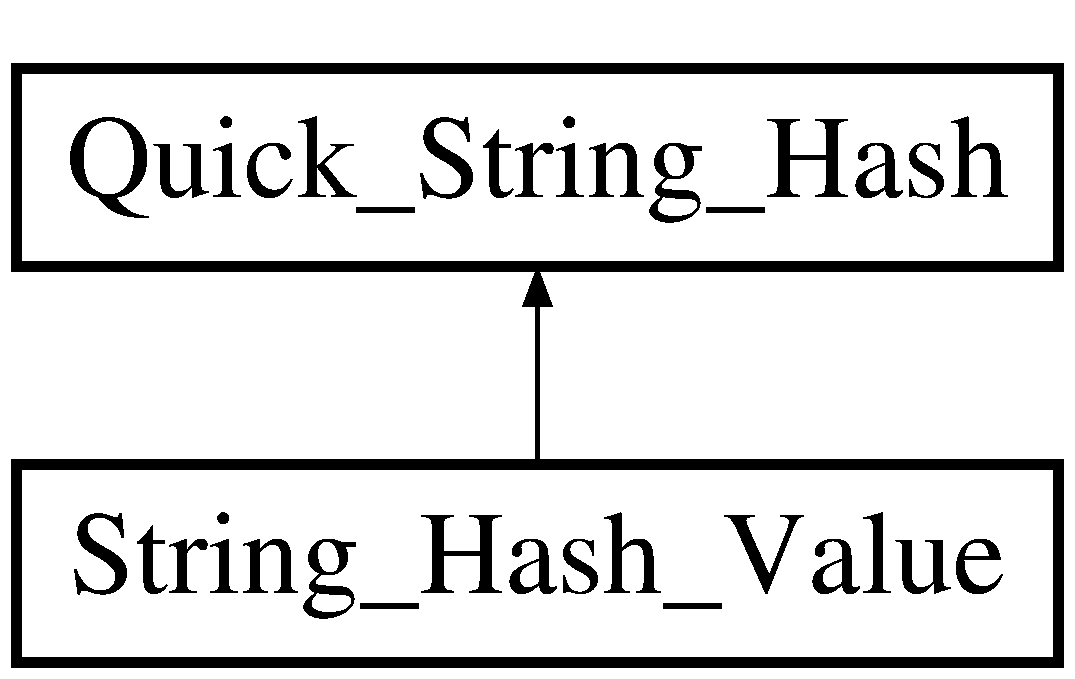
\includegraphics[height=2cm]{classQuick__String__Hash}
\end{center}
\end{figure}
\subsection*{Public Methods}
\begin{CompactItemize}
\item 
{\bf Quick\_\-String\_\-Hash} ()
\item 
{\bf $\sim$Quick\_\-String\_\-Hash} ()
\item 
Quick\_\-String\_\-Hash \& {\bf insert} (const char $\ast$s)
\item 
Quick\_\-String\_\-Hash \& {\bf operator$<$$<$} (const char $\ast$s)
\item 
int {\bf read} (const char $\ast$s) const
\item 
int {\bf operator[$\,$]} (const char $\ast$s) const
\item 
unsigned long {\bf nodes} () const
\item 
unsigned long {\bf size} () const
\end{CompactItemize}
\subsection*{Protected Methods}
\begin{CompactItemize}
\item 
Quick\_\-String\_\-Hash $\ast$ {\bf add\_\-list\_\-element} (int i)
\end{CompactItemize}
\subsection*{Protected Attributes}
\begin{CompactItemize}
\item 
Quick\_\-String\_\-Hash $\ast$$\ast$ {\bf list}
\item 
int {\bf offset}
\item 
int {\bf len}
\end{CompactItemize}


\subsection{Constructor \& Destructor Documentation}
\index{Quick_String_Hash@{Quick\_\-String\_\-Hash}!Quick_String_Hash@{Quick\_\-String\_\-Hash}}
\index{Quick_String_Hash@{Quick\_\-String\_\-Hash}!Quick_String_Hash@{Quick\_\-String\_\-Hash}}
\subsubsection{\setlength{\rightskip}{0pt plus 5cm}Quick\_\-String\_\-Hash::Quick\_\-String\_\-Hash ()\hspace{0.3cm}{\tt  [inline]}}\label{classQuick__String__Hash_a0}




Definition at line 187 of file dil2al.hh.

References len, and offset.

Referenced by add\_\-list\_\-element(), and insert().



\footnotesize\begin{verbatim}187 : list(NULL), offset(0), len(0) {}
\end{verbatim}\normalsize 
\index{Quick_String_Hash@{Quick\_\-String\_\-Hash}!~Quick_String_Hash@{$\sim$Quick\_\-String\_\-Hash}}
\index{~Quick_String_Hash@{$\sim$Quick\_\-String\_\-Hash}!Quick_String_Hash@{Quick\_\-String\_\-Hash}}
\subsubsection{\setlength{\rightskip}{0pt plus 5cm}Quick\_\-String\_\-Hash::$\sim$Quick\_\-String\_\-Hash ()\hspace{0.3cm}{\tt  [inline]}}\label{classQuick__String__Hash_a1}




Definition at line 189 of file dil2al.hh.

References len.



\footnotesize\begin{verbatim}189 { if (list) { for (int i=0; i<len; i++) delete list[i]; delete[] list; } }
\end{verbatim}\normalsize 


\subsection{Member Function Documentation}
\index{Quick_String_Hash@{Quick\_\-String\_\-Hash}!add_list_element@{add\_\-list\_\-element}}
\index{add_list_element@{add\_\-list\_\-element}!Quick_String_Hash@{Quick\_\-String\_\-Hash}}
\subsubsection{\setlength{\rightskip}{0pt plus 5cm}Quick\_\-String\_\-Hash $\ast$ Quick\_\-String\_\-Hash::add\_\-list\_\-element (int {\em i})\hspace{0.3cm}{\tt  [protected]}}\label{classQuick__String__Hash_b0}




Definition at line 179 of file utilities.cc.

References len, list, offset, and Quick\_\-String\_\-Hash().

Referenced by insert(), and String\_\-Hash\_\-Value::insert\_\-value().



\footnotesize\begin{verbatim}179                                                              {
180 // Note: currently there is no way for this to return NULL, since allocation
181 // errors are not caught.
182         if (i<0) i = 0; // reduce the impact of roll-over errors
183         if (!list) { // allocate list of pointers
184                 len = 1;
185                 list = new Quick_String_Hash*[len];
186 #ifdef CONST_QUICK_STRING_HASH_ENDNODE
187                 list[0] = const_cast<Quick_String_Hash *>(&_qsh_endnode);
188 #else
189                 list[0] = new Quick_String_Hash();
190 #endif
191                 offset = i;
192                 return list[0];
193         }
194         if (i<offset) { // prepend to the list
195                 int oldlen = len;
196                 len += (offset-i);
197                 offset = i;
198                 Quick_String_Hash ** oldlist = list;
199                 list = new Quick_String_Hash*[len];
200                 for (int j = 0; j<len; j++) list[j] = NULL; // initialize list
201 #ifdef CONST_QUICK_STRING_HASH_ENDNODE
202                 list[0] = const_cast<Quick_String_Hash *>(&_qsh_endnode);
203 #else
204                 list[0] = new Quick_String_Hash();
205 #endif
206                 for (int j = oldlen-1, k = len-1; j>=0; j--, k--) list[k] = oldlist[j];
207                 delete[] oldlist;
208                 return list[0];
209         }
210         i -= offset;
211         if (i>=len) { // append to the list
212                 int oldlen = len;
213                 len = i+1;
214                 Quick_String_Hash ** oldlist = list;
215                 list = new Quick_String_Hash*[len];
216                 for (int j = 0; j<len; j++) list[j] = NULL; // initialize list
217 #ifdef CONST_QUICK_STRING_HASH_ENDNODE
218                 list[i] = const_cast<Quick_String_Hash *>(&_qsh_endnode);
219 #else
220                 list[i] = new Quick_String_Hash();
221 #endif
222                 for (int j = 0; j<oldlen; j++) list[j] = oldlist[j];
223                 delete[] oldlist;
224                 return list[i];
225         }
226         if (!list[i]) { // add list element
227 #ifdef CONST_QUICK_STRING_HASH_ENDNODE
228                 list[i] = const_cast<Quick_String_Hash *>(&_qsh_endnode);
229 #else
230                 list[i] = new Quick_String_Hash();
231 #endif
232                 return list[i];
233         }
234 }
\end{verbatim}\normalsize 
\index{Quick_String_Hash@{Quick\_\-String\_\-Hash}!insert@{insert}}
\index{insert@{insert}!Quick_String_Hash@{Quick\_\-String\_\-Hash}}
\subsubsection{\setlength{\rightskip}{0pt plus 5cm}Quick\_\-String\_\-Hash \& Quick\_\-String\_\-Hash::insert (const char $\ast$ {\em s})}\label{classQuick__String__Hash_a2}




Definition at line 236 of file utilities.cc.

References add\_\-list\_\-element(), len, list, offset, and Quick\_\-String\_\-Hash().

Referenced by String\_\-Hash\_\-Value::insert\_\-value(), and operator$<$$<$().



\footnotesize\begin{verbatim}236                                                             {
237 // *** can adapt this to the faster method according to results obtained with read and read_recursive
238         if (s[0]=='\0') return (*this);
239         int i = ((int) s[0]);   // implied list coordinate
240         int r = i - offset;             // real list coordinate
241         if (r<0) {
242                 if (add_list_element(i)==NULL) return (*this);
243                 r = i - offset; // adjust to new offset
244         } else if (r>=len) {
245                 if (add_list_element(i)==NULL) return (*this); // this also takes care of the case where the list is unallocated
246                 r = i - offset; // adjust to new offset
247         } else if (!list[r]) {
248                 if (add_list_element(i)==NULL) return (*this);
249         }
250 #ifdef CONST_QUICK_STRING_HASH_ENDNODE
251         if ((s[1]!='\0') && (list[r]==&_qsh_endnode)) list[r] = new Quick_String_Hash(); // allocate so that list can be made
252 #endif
253         list[r]->insert(&s[1]);
254         return (*this);
255 }
\end{verbatim}\normalsize 
\index{Quick_String_Hash@{Quick\_\-String\_\-Hash}!nodes@{nodes}}
\index{nodes@{nodes}!Quick_String_Hash@{Quick\_\-String\_\-Hash}}
\subsubsection{\setlength{\rightskip}{0pt plus 5cm}unsigned long Quick\_\-String\_\-Hash::nodes () const}\label{classQuick__String__Hash_a6}




Definition at line 284 of file utilities.cc.

References len, list, and res.



\footnotesize\begin{verbatim}284                                              {
285 #ifdef CONST_QUICK_STRING_HASH_ENDNODE
286         if (this==&_qsh_endnode) return 0;
287 #endif
288         unsigned long res = 1;
289         for (int i=0; i<len; i++) if (list[i]) res += list[i]->nodes();
290         return res;
291 }
\end{verbatim}\normalsize 
\index{Quick_String_Hash@{Quick\_\-String\_\-Hash}!operator<<@{operator$<$$<$}}
\index{operator<<@{operator$<$$<$}!Quick_String_Hash@{Quick\_\-String\_\-Hash}}
\subsubsection{\setlength{\rightskip}{0pt plus 5cm}Quick\_\-String\_\-Hash\& Quick\_\-String\_\-Hash::operator$<$$<$ (const char $\ast$ {\em s})\hspace{0.3cm}{\tt  [inline]}}\label{classQuick__String__Hash_a3}




Definition at line 192 of file dil2al.hh.

References insert().



\footnotesize\begin{verbatim}192 { return insert(s); }
\end{verbatim}\normalsize 
\index{Quick_String_Hash@{Quick\_\-String\_\-Hash}!operator[]@{operator[]}}
\index{operator[]@{operator[]}!Quick_String_Hash@{Quick\_\-String\_\-Hash}}
\subsubsection{\setlength{\rightskip}{0pt plus 5cm}int Quick\_\-String\_\-Hash::operator[$\,$] (const char $\ast$ {\em s}) const\hspace{0.3cm}{\tt  [inline]}}\label{classQuick__String__Hash_a5}




Definition at line 194 of file dil2al.hh.

References read().



\footnotesize\begin{verbatim}194 { return read(s); }
\end{verbatim}\normalsize 
\index{Quick_String_Hash@{Quick\_\-String\_\-Hash}!read@{read}}
\index{read@{read}!Quick_String_Hash@{Quick\_\-String\_\-Hash}}
\subsubsection{\setlength{\rightskip}{0pt plus 5cm}int Quick\_\-String\_\-Hash::read (const char $\ast$ {\em s}) const}\label{classQuick__String__Hash_a4}




Definition at line 258 of file utilities.cc.

References len, list, and offset.

Referenced by Search\_\-Target::check\_\-encountered(), and operator[$\,$]().



\footnotesize\begin{verbatim}258                                                 {
259         // Determines if the next character in s exists in the tree
260         if (s[0]=='\0') return 1;
261         int i = ((int) s[0]);   // implied list coordinate
262         if (i<offset) return 0;
263         i -= offset;                    // real list coordinate
264         if (i>=len) return 0;   // this also takes care of the case where the list is unallocated
265         if (list[i]) return list[i]->read(&s[1]);
266         return 0;
267 }
\end{verbatim}\normalsize 
\index{Quick_String_Hash@{Quick\_\-String\_\-Hash}!size@{size}}
\index{size@{size}!Quick_String_Hash@{Quick\_\-String\_\-Hash}}
\subsubsection{\setlength{\rightskip}{0pt plus 5cm}unsigned long Quick\_\-String\_\-Hash::size () const}\label{classQuick__String__Hash_a7}




Definition at line 293 of file utilities.cc.

References len, list, and res.



\footnotesize\begin{verbatim}293                                             {
294 #ifdef CONST_QUICK_STRING_HASH_ENDNODE
295         if (this==&_qsh_endnode) return 0;
296 #endif
297         unsigned long res = sizeof(*this);
298         for (int i=0; i<len; i++) if (list[i]) res += list[i]->size();
299         return res;
300 }
\end{verbatim}\normalsize 


\subsection{Member Data Documentation}
\index{Quick_String_Hash@{Quick\_\-String\_\-Hash}!len@{len}}
\index{len@{len}!Quick_String_Hash@{Quick\_\-String\_\-Hash}}
\subsubsection{\setlength{\rightskip}{0pt plus 5cm}int Quick\_\-String\_\-Hash::len\hspace{0.3cm}{\tt  [protected]}}\label{classQuick__String__Hash_n2}




Definition at line 183 of file dil2al.hh.

Referenced by add\_\-list\_\-element(), insert(), String\_\-Hash\_\-Value::insert\_\-value(), nodes(), Quick\_\-String\_\-Hash(), read(), String\_\-Hash\_\-Value::read\_\-value(), size(), and $\sim$Quick\_\-String\_\-Hash().\index{Quick_String_Hash@{Quick\_\-String\_\-Hash}!list@{list}}
\index{list@{list}!Quick_String_Hash@{Quick\_\-String\_\-Hash}}
\subsubsection{\setlength{\rightskip}{0pt plus 5cm}Quick\_\-String\_\-Hash$\ast$$\ast$ Quick\_\-String\_\-Hash::list\hspace{0.3cm}{\tt  [protected]}}\label{classQuick__String__Hash_n0}




Definition at line 181 of file dil2al.hh.

Referenced by add\_\-list\_\-element(), insert(), String\_\-Hash\_\-Value::insert\_\-value(), nodes(), read(), String\_\-Hash\_\-Value::read\_\-value(), and size().\index{Quick_String_Hash@{Quick\_\-String\_\-Hash}!offset@{offset}}
\index{offset@{offset}!Quick_String_Hash@{Quick\_\-String\_\-Hash}}
\subsubsection{\setlength{\rightskip}{0pt plus 5cm}int Quick\_\-String\_\-Hash::offset\hspace{0.3cm}{\tt  [protected]}}\label{classQuick__String__Hash_n1}




Definition at line 182 of file dil2al.hh.

Referenced by add\_\-list\_\-element(), insert(), String\_\-Hash\_\-Value::insert\_\-value(), Quick\_\-String\_\-Hash(), read(), and String\_\-Hash\_\-Value::read\_\-value().

The documentation for this class was generated from the following files:\begin{CompactItemize}
\item 
{\bf dil2al.hh}\item 
{\bf utilities.cc}\end{CompactItemize}
